\section{Case Study: Modularizing Components in a Small Scripting Language}

%This section shows the expressiveness of \name. 
%We show that features of \name
%(dynamically composable traits, intersection types, the merge operator,
%parametric polymorphism and disjoint quantification) enable extensible designs
%that have been presented in mainstream languages. 
%In particular, \name addresses
%limitations of those languages, making the designs significantly
%simpler. 
To further illustrate the applicability of \name, we present a case study based
on the approach to Object Algebras presented in Section~\ref{sec:OA}. The case
study modularizes several orthogonal features of a subset of JavaScript, used
by~\citet{poplcook} in his undergraduate textbook on programming languages. The
case study illustrates how various features and operations can be modularly
developed and later composed to assemble a complete language with various
operations baked in.


% The second is a case study on embedding a higher-order
% domain-specific language (simply-typed lambda-calculus with conditional and
% constants) with a selectable evaluation order: CBN and CBV. The outcome is an
% evaluator parameterized over the evaluation order. This case study shows that
% features of \name are sufficient for such a seemingly impossible task, which
% usually require fancy types (in particular, GADTs).

\subsection{Overview}

Figure~\ref{fig:mini-js} presents the syntax of the expressions, values and
types provided by the features; each line is annotated with the corresponding
feature. Starting from a simple arithmetic language, we gradually introduce new
features and combine them with some of the existing features to form various
languages. Below we briefly explain what constitutes each feature:
\begin{itemize}
\item $\mathit{Arith}$ contains numerical literals, addition, subtraction, among
  others.
\item $\mathit{Bool}$ introduces Boolean values, comparison, and if expressions.
\item $\mathit{Var}$ introduces local variables and variable declarations.
\item $\mathit{Function}$ introduces top-level functions and function calls.
\end{itemize}

% For each feature, we also define three operations: evaluator, pretty printer,
% and type checker.

\begin{figure}[t]
\centering
% \begin{small}
\begin{tabular}{lrclr}
  Expressions & $e$ & ::= & $[[N]] \mid [[e1 + e2]] \mid [[e1 - e2]] \mid [[e1 * e2]] \mid [[e1 / e2]] $ & $\mathit{Arith}$ \\
              && $\mid$ & $[[BL]] \mid [[e1 == e2]] \mid [[e1 < e2]] \mid$ $[[if e1 then e2 else e3]] $ & $\mathit{Bool}$\\
              && $\mid$ & $[[x]] \mid [[var x = e1 ; e2]]$  &  $\mathit{Var}$ \\
  Programs & $[[jpgm]]$ & ::= & $[[jdecl1 .. jdecln e]]$ & $\mathit{Function}$ \\
  Functions & $[[jdecl]]$ & ::= & $[[function f ( x : t ) { e }]]$ & \\
  Values & $v$ & ::= & $[[N]] \mid [[BL]]$ & \\
  Types  & $t$ & ::= & $[[int]] \mid [[bool]]$ &
\end{tabular}
% \end{small}
\caption{Mini-JS expressions, values, and types}
\label{fig:mini-js}
\end{figure}

% \bruno{You should explain the four features.} \jeremy{done}

% \bruno{The next 4 subsection {\bf are not what we want to see in a
%     case study section}. Repeating the same ideas that were already
%   presented in Section~4 is pointless, and that's what you are doing
%   here. In a case study you want to measure, evaluate the benefits of
%   modularity. For example in terms of SLOC, or how many languages can
%   you recover from the components that we have; how many lines are
%   required to recover each languages, etc. Please go and have a look
%   at Case Study sections of other papers. I suggest ``Scrap your
%   Boilerplate as Object Algebras''; and "Meta-theory a la Carte". Also
% Weixin's case study on EVF is pretty good.}
% \bruno{Also I think you could talk about the subtyping/inheritance
%   relations of the languages that you can assemble. Perhaps draw some
% diagrams. }

Figure~\ref{fig:dependency} gives an overview of the reusable components of the
implementation, and the subtyping/inheritance relations of the languages we can
assemble. The interactions between languages and features are revealed by the
arrows. Below we briefly explain what features/operations each language supports:
\begin{itemize}
\item \lstinline{ArithL} is a simple language of arithmetic expressions,
  directly inherited from the feature $\mathit{Arith}$. We define an evaluator
  and a pretty printer.
\item \lstinline{BoolArithL} extends \lstinline{ArithL} with the feature
  $\mathit{Bool}$. Apart from the evaluator and pretty printer, we define
  another operation: type checker. Thus \lstinline{BoolArithL} is illustrative
  of solving the Expression Problem.
\item \lstinline{VarArithL} extends \lstinline{BoolArithL} with the feature
  $\mathit{Var}$. We define an evaluator, a pretty printer, and a type checker.
\item \lstinline{Mini-JS} is the complete language that inherits all the
  features and operations.
\end{itemize}

\noindent Figure~\ref{fig:dependency} also illustrates the subtyping/inheritance
relations between each language. For example, the leftward arrow between
\lstinline{BoolArithL} and \lstinline{ArithL} says that \lstinline{BoolArithL}
extends \lstinline{ArithL}, while the rightward dashed arrow between them says
that \lstinline{ArithL} is a subtype of \lstinline{BoolArithL}. We thus obtain 4
languages and 11 operations in total.

\begin{figure}[t]
  \centering
  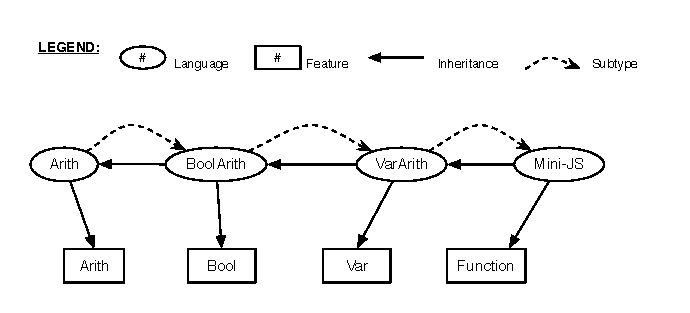
\includegraphics{dependency.eps}
  \caption{Overview of the language components.}
  \label{fig:dependency}
\end{figure}

\subsection{Evaluation}

To evaluate \name's implementation of the case study, Figure~\ref{fig:sloc}
compares the number of source lines of code (SLOC, lines of code without
counting empty lines and comments) for \name's implementation with the vanilla
AST-based implementation in Haskell. Since Haskell is a more concise language
than \name, we omit lines of code that are for infrastructure purpose. In the
left part, for each feature, we count lines of the Object Algebra interface, and
the Object Algebras for the operations. In the right part, for each language, we
count lines of defining the AST, and the code to combine previously defined
operations. For example, here is the code that is needed to make the
\lstinline{VarArithL} language that extends \lstinline{BoolArithL} with the
$\mathit{Var}$ feature.

\lstinputlisting[linerange=383-394]{../examples/case_study1.txt}% APPLY:linerange=VARARITHL

\noindent As we can see, there are 2 lines of code to define the AST, and 6
lines of code to combine the operations. Thus for \lstinline{VarArithL} we only
need 8 lines in total.

Therefore, the total number of the \name's implementation is the sum of all the
lines in the feature and language parts. Although \name is considerably more
verbose than a functional language like Haskell, \name's implementation for all
4 languages in total reduces approximately 33\% in terms of SLOC. The reason is
that, the more frequently a feature is reused by other languages directly or
indirectly, the more reduction we see in the total SLOC. For example,
$\mathit{Arith}$ is used across all 4 languages. Even though \lstinline{ArithL}
itself alone has a lot more SLOC ($40 = 37+3$) than that of Haskell (which has
29), we still get a huge gain when implementing other languages.



\begin{figure}[t]
  \centering
  \begin{tabular}{lc|lccc}
    \hline
    \bf{Feature} & \name & \bf{Language} & \name & \bf{Haskell} & \bf{\% Reduced}  \\
    \hline
    $\mathit{Arith}$ & 37 & \lstinline$ArithL$ & 3 & 29 & 90\%  \\
    $\mathit{Bool}$ & 66 & \lstinline$BoolArithL$ & 44 & 86 & 49\% \\
    $\mathit{Var}$ & 22 & \lstinline$VarArithL$ & 8 & 99 & 92\% \\
    $\mathit{Function}$ & 24 & \lstinline$Mini-JS$ & 20 & 120 & 83\% \\
    \hline
    \bf{Total} & & & 224 & 334 & 33\% \\
    \hline

  \end{tabular}
  \caption{SLOC statistics: \name implementation vs vanilla AST implementation.}
  \label{fig:sloc}
\end{figure}


\begin{comment}

\subsection{The Base Language (Arith)}

We start with a very simple language of arithmetic expressions, as shown on the
left hand side of Figure~\ref{fig:base-lang}. The base language has features
such as literals, addition, subtraction among others. As with examples in
Section~\ref{sec:extensibility}, we use visitors to encode datatypes. The
right hand side of Figure~\ref{fig:base-lang} defines the interfaces of the
operations.

\begin{figure}[t]
  \centering
  \begin{tabular}{cc}
    \begin{subfigure}[t]{0.45\textwidth}
      \centering
      \lstinputlisting[linerange=-]{}% APPLY:linerange=BASE_DEF
    \end{subfigure}
    &
    \begin{subfigure}[t]{0.45\textwidth}
      \centering
      \lstinputlisting[linerange=-]{}% APPLY:linerange=INTERFACE
    \end{subfigure}
  \end{tabular}
  \caption{The base language (left) and the interfaces of the operations (right)}
  \label{fig:base-lang}
\end{figure}

\subsubsection{Evaluator}

The evaluation interface (\lstinline{IEval}) contains the \lstinline{eval}
method, which is a function from an evaluation environment (\lstinline{Env}) to
\lstinline{Maybe[Value]}. At this stage, the evaluation environment is not used,
but will be useful when we have variables. The evaluation of the base language
is quite straightforward, so we only show part of the code below:
\lstinputlisting[linerange=-]{}% APPLY:linerange=BASE_EVALUATOR
To reduce boilerplate code when dealing with \lstinline{Maybe} values, like in
Haskell, we encode the bind operator \lstinline{bind} of the \lstinline{Maybe}
monad.

\subsubsection{Pretty printer and type checker}

Pretty printer and type checker are constructed in a similar manner, as is shown
in Figure~\ref{fig:printer} and~\ref{fig:checker}.

\begin{figure}[t]
  \centering
  \lstinputlisting[linerange=-]{}% APPLY:linerange=PRETTY_BASE
  \caption{An object algebra for pretty printing. }
  \label{fig:printer}
\end{figure}

\begin{figure}[t]
  \centering
  \lstinputlisting[linerange=-]{}% APPLY:linerange=TYPECHECKER_BASE
  \caption{An object algebra for type checking. }
  \label{fig:checker}
\end{figure}


\subsection{Adding Conditional Expressions (Bool)}

Now we extend the base language with conditional expressions.
\lstinputlisting[linerange=-]{}% APPLY:linerange=CONDITIONAL
The augmented language now has Boolean literals, comparison features
(\lstinline{eq} and \lstinline{le}) and if expressions.

We omit the code of the operations as they follow the same pattern as we
described in Section~\ref{sec:extensibility}.

% Here is the extended evaluator. Now we need Boolean values.
% \lstinputlisting[linerange=-]{}% APPLY:linerange=EVALUATOR_CONDITIONAL
% Note that we didn't touch anything from \lstinline{evalArithAlg} but extend it
% to from a new evaluator. Now because the language can produce two kinds of
% values, it is worth noting that \lstinline{fromNum} (or \lstinline{fromBool}) is
% partial, meaning that it can diverge at run-time if the value is not a number
% (or Boolean). This is why we need a type checker to make sure such things cannot
% happen at run-time.

% Same goes for the pretty printer and the type checker.
% \lstinputlisting[linerange=-]{}% APPLY:linerange=PRETTY_CONDITIONAL
% \lstinputlisting[linerange=-]{}% APPLY:linerange=TYPECHECKER_CONDITIONAL



\subsection{Adding Variable Declarations (Var)}

Next we extend our language again with local variables and variable
declarations. We add two new constructors \lstinline{var} and \lstinline{decl}.
\lstinputlisting[linerange=-]{}% APPLY:linerange=VARIABLE
For simplicity, we encode variables using strings. \lstinline{decl} takes three
arguments, the first is the variable to be declared, the second is the
expression bound with the variable, and the third is the body within which the
declared variable is in scope. Now the language is interesting enough to express
something like \lstinline{var x = 3; x + 1}.

The evaluator finally makes use of the evaluation environment, which is a
mapping from variables to values.
\lstinputlisting[linerange=-]{}% APPLY:linerange=EVALUATOR_VARIABLE
For the variable case, we look it up in the environment to find its bound value.
For the declaration case, we evaluate the body expression in the augmented
environment.

We omit the code of pretty printer and type checker for the space reason.

\subsection{Adding Top-level Functions (Function)}

We add, as the final piece, top-level functions to the language. The only
extension is a call expression that takes a function name and an actual
argument expression\footnote{For simplicity, we only allow functions with one
  argument.}.
\lstinputlisting[linerange=-]{}% APPLY:linerange=TOP_LEVEL

Top-level functions are collected into a function environment, a list of
bindings of function names to function definitions. A program is then a function
environment together with a main expression. We omit the code here, and refer an
interested reader to the supplementary materials.

\end{comment}


% \bruno{I think the part of the following is the only thing that should
% that could be mentioned here, in a discussion about what does it take
% to assemble a language from components. } \jeremy{done}

\subsection{Putting all together}

% With all the components ready, we can assemble them at will to cook a language
% with whatever features we want. For example, we hope by now the reader can share
% our feeling that this is indeed a simple and modular way to cook a language
% incrementally.

To demonstrate the usage of the final language \lstinline{MiniJS}, here is a function that
makes sure ``well-typed programs cannot go wrong'':
\lstinputlisting[linerange=498-504]{../examples/case_study1.txt}% APPLY:linerange=SUPER_DEF
It type checks the program before passing it to the evaluator and pretty
printer.

% we first create a program that
% uses all the features the language supports now.
% \lstinputlisting[linerange=-]{}% APPLY:linerange=FINAL_TEST
% The concrete syntax of the program is shown in the comment above. We assume a
% pre-defined function environment (\lstinline{fenv}) containing the definition of
% the \lstinline{add1} function.

% Finally we apply it to the program we have just created:
% \lstinputlisting[linerange=508-509]{../examples/case_study1.txt}% APPLY:linerange=TEST_TEST
% Everything works as expected!


\begin{comment}
\subsection{Parameterizing Expressions by the Evaluation Order}

We now turn to the second case study. In this case study, we embed a
higher-order domain-specific language inside \name. Our object language in this
case study is typed lambda calculus with conditional and constants. This time,
the embedding not only demonstrates the extensibility, as is shown in the first
case study, but also object types, expressed in the meta-language (\name) and
manifestly ensuring well-scoped and well-typed expressions in the object
language. What is more, the evaluator over the object expressions is type
preserving by construction. The embedding of typed languages is directly
inspired by Kiselyov's lecture notes~\cite{kiselyov2012typed} on the
"tagless-final" approach to embedding languages.

\paragraph{Well-typed object expressions} One important issue with such
embedding is how to deal with binders in the object language. In general there
are two options, one can either use deBrujin indices~\cite{}, or higher-order
abstract syntax (HOAS)~\cite{}. Each option has its cons and pros, but for this
particular case study, we find HOAS convenient. HOAS represents object language
abstractions as \name abstractions and object variables as \name variables. By
utilizing the infrastructure of the meta-language, we are free of issues such as
variable capture. Here is the interface of the object language.
\lstinputlisting[linerange=24-29]{../examples/case_study2.txt}% APPLY:linerange=TYPED_LAMBDA
Embedded object expressions of type \lstinline{A} are represented as \name
values of the type \lstinline{Expr[A]}. The \lstinline{bot} constructor, which
represents non-terminating computation, is there for the purpose of illustrating
different evaluation strategies.

A careful reader may notice that the \lstinline{ExprAlg} interface has no
abstractions. This is intentional! Evaluators with different evaluation
strategies only differ in the interpretation for abstractions, as will be shown
later on. For this reason, \lstinline{lam} is moved to a separate interface of
its own.
\lstinputlisting[linerange=16-18]{../examples/case_study2.txt}% APPLY:linerange=ABSTRACTION


\paragraph{Well-typed evaluator}
The benefit of typeful embedding shows up when defining the evaluator.
\lstinputlisting[linerange=33-38]{../examples/case_study2.txt}% APPLY:linerange=TYPED_EVAL
Unlike the evaluator in the first case study, there is no need for a separate
\lstinline{Value} datatype for values, as they are directly modeled by \name
values. Note that the resulting evaluator is \textit{type preserving} by
construction.

\paragraph{Call-by-name, call-by-value}
Our evaluator defined in the first case study inherits the evaluation strategy
from the meta-language. We now show call-by-name and call-by-value evaluators.
The two evaluators are quite alike, sharing most of the code. As said before,
the only difference is the interpretation for \lstinline{lam}.
\lstinputlisting[linerange=68-73]{../examples/case_study2.txt}% APPLY:linerange=CBN_CBV
The call-by-name \lstinline{lam}, when applied, will receive an unevaluated
argument expression, use it as it is. The call-by-value \lstinline{lam}, as in
the call-by-name evaluator, receives an unevaluated argument expression,
evaluates it before passing its result to the abstraction body \lstinline{f}.

Now to make an evaluator parameterized over the evaluation order, we just take a
trait \lstinline{o} with unknown implementation, compose it with other language
features.
\lstinputlisting[linerange=82-83]{../examples/case_study2.txt}% APPLY:linerange=MAKE_EVAL
Here is the call-by-name evaluator at work:
\lstinputlisting[linerange=88-93]{../examples/case_study2.txt}% APPLY:linerange=CBN_TEST
On the other hand, \lstinline{(evaluator evalBindCBV ex)()} would result in a
infinite loop. The complete code with several examples can be found in the
supplementary materials.

\jeremy{I am afraid we don't seem to have many advantages over OCaml's version,
  because we don't really have higher-kinded types, we cannot make a AST type
  for this example, though \lstinline{makeEvaluator} seems to be one advantage }

\end{comment}